% !TEX program = xelatex
\documentclass[11pt,a4paper]{article}
\usepackage{amsmath,amssymb}
\usepackage{graphicx}
\graphicspath{{figures/}}
\usepackage{geometry}
\usepackage{hyperref}
\usepackage{xcolor}
\usepackage{booktabs}
\usepackage{longtable}
\usepackage{listings}
\usepackage{fontspec}
\usepackage{xeCJK}
\geometry{margin=25mm}
\IfFontExistsTF{HaranoAjiMincho-Regular.otf}{%
  \setCJKmainfont[AutoFakeBold=2.5]{HaranoAjiMincho-Regular.otf}%
  \setCJKsansfont[AutoFakeBold=2.5]{HaranoAjiGothic-Regular.otf}%
}{%
  \IfFontExistsTF{Noto Serif CJK JP}{%
    \setCJKmainfont{Noto Serif CJK JP}%
    \setCJKsansfont{Noto Sans CJK JP}%
  }{%
    \IfFontExistsTF{Hiragino Mincho ProN}{%
      \setCJKmainfont{Hiragino Mincho ProN}%
      \setCJKsansfont{Hiragino Sans}%
    }{%
      \setCJKmainfont[AutoFakeBold=2.5]{IPAMincho}%
      \setCJKsansfont[AutoFakeBold=2.5]{IPAGothic}%
    }%
  }%
}
\hypersetup{colorlinks=true,linkcolor=blue,urlcolor=blue,citecolor=blue,pdftitle={OpenAyane Implementation Plan},pdfauthor={Tomoyuki Kano}}
\lstset{basicstyle=\ttfamily\small,breaklines=true,frame=single}
\title{OpenAyaneの実装計画\\\large RDE評価器に基づく意味変化監査機構の設計と段階的実装}
\author{Tomoyuki Kano\\ZYX Corp 株式会社 人工叡智研究室\\Independent Researcher\\ORCID: \href{https://orcid.org/0009-0004-8213-4631}{0009-0004-8213-4631}}
\date{Version 1.0（2026-05-04）}
\begin{document}
\maketitle

\begin{center}
Copyright \copyright{} 2026 Tomoyuki Kano.\\
This paper is licensed under the Creative Commons Attribution 4.0 International License (CC BY 4.0).
\end{center}

\begin{abstract}
本稿は、OpenAyaneを、生成AIおよびエージェント型AIの出力・編集・実行過程における意味変化を監査する実装可能な機構として定式化する。大規模言語モデルは、文書やコードを厳密に保存しながら局所変更する機械ではなく、入力、履歴、指示、文脈に基づいて対象を再生成する。そのため、表面的には自然に見える出力の内部で、定義、制約、数値、参照、論旨、依存関係が静かに変化することがある。本稿ではこの現象をSilent $\Delta M$と呼び、RDE（Resonant Deviation Evaluator）を中核評価器として導入する。RDEはDiff、Policy Filter、Validator、LLM Evaluatorそのものではなく、変換前状態、期待された変換、実際の生成結果の差異を、タスク契約、文脈、関係履歴、制度的制約と照合し、意味変化の許可性と危険性を分類する評価器である。一方、OpenAyaneはRDEを含み、Task Contract生成、Generator制御、Structural Diff、Semantic Delta、Policy Bridge、Safe Execution Runtime、AuditLog、RelationStore更新、履歴参照ループを統合する関係的制御機構である。
\end{abstract}

\noindent\textbf{キーワード：} OpenAyane, RDE, Resonant Deviation Evaluator, Silent $\Delta M$, 意味変化監査, Agent Safety, Relation Store

\section{はじめに}
生成AIへの委任が進むにつれ、「一部だけ直す」「主張を変えずに整える」「アルゴリズムを変えずにエラー処理を追加する」といった依頼において、表面上は自然でありながら、意味上重要な要素が静かに変化する問題が顕在化している。本稿では、この未署名の意味変化をSilent $\Delta M$と呼ぶ。問題は、変化そのものではない。問題は、その変化が許可され、署名され、検証可能で、必要に応じて差し戻し可能であるかである。

\section{RDEとOpenAyaneの役割分担}
本稿では、RDEとOpenAyaneを明確に区別する。RDEは、生成系またはエージェント系が生む意味変化$\Delta M$を評価し、その変化が保存、許可された逸脱、軽微な副次的変化、疑義ある逸脱、重大な腐食、創造的逸脱のいずれに属するかを分類する評価器である。

一方、OpenAyaneはRDEそのものではない。OpenAyaneは、RDEを中核評価器として組み込み、Task Contract生成、Generator制御、Structural Diff、Semantic Delta、Policy Bridge、Safe Execution Runtime、AuditLog、RelationStore更新、履歴参照ループを統合する機構である。したがって、RDEの問いは「この意味変化は何か」であり、OpenAyaneの問いは「その評価結果を、どの制度的・関係的制御ループの中で、どのように扱うか」である。

\section{形式モデル}
文書または状態を$D_t$、意味写像を$M(D_t)$、許可された変換を$A_t$、実際の生成器による変換を$\hat{A}_t$とする。期待される意味状態は
\[
M_t^* = M(A_t(D_{t-1}))
\]
であり、実際の意味状態は
\[
\hat{M}_t = M(\hat{A}_t(D_{t-1}))
\]
である。意味逸脱は
\[
\Delta M_t = \hat{M}_t - M_t^*
\]
として表される。ただし、RDEの目的は$\|\Delta M_t\|$を単純に最小化することではない。創造的変換や設計変更では、大きな$\Delta M$が正当な場合がある。RDEの目的は、$\Delta M$の大きさ、方向、対象、許可性、可逆性、検証可能性、制度的署名性を評価することである。

\section{OpenAyaneの実装フロー}
OpenAyaneの実装フローは、単線的な生成・評価・実行パイプラインではない。各実行後にAuditLogへ記録されたTask Contract、Structural Diff、Semantic Delta、RDE分類、Policy決定、Rollback、人間レビュー結果はRelationStoreへ集約され、trust、stability、context\_affinity、drift pattern、generator reliability、document fragilityとして再構成される。これらの履歴状態は、次回以降のIntent解析、Task Contract生成、RDE判定、Policy判断に再入力される。

\begin{figure}[htbp]
  \centering
  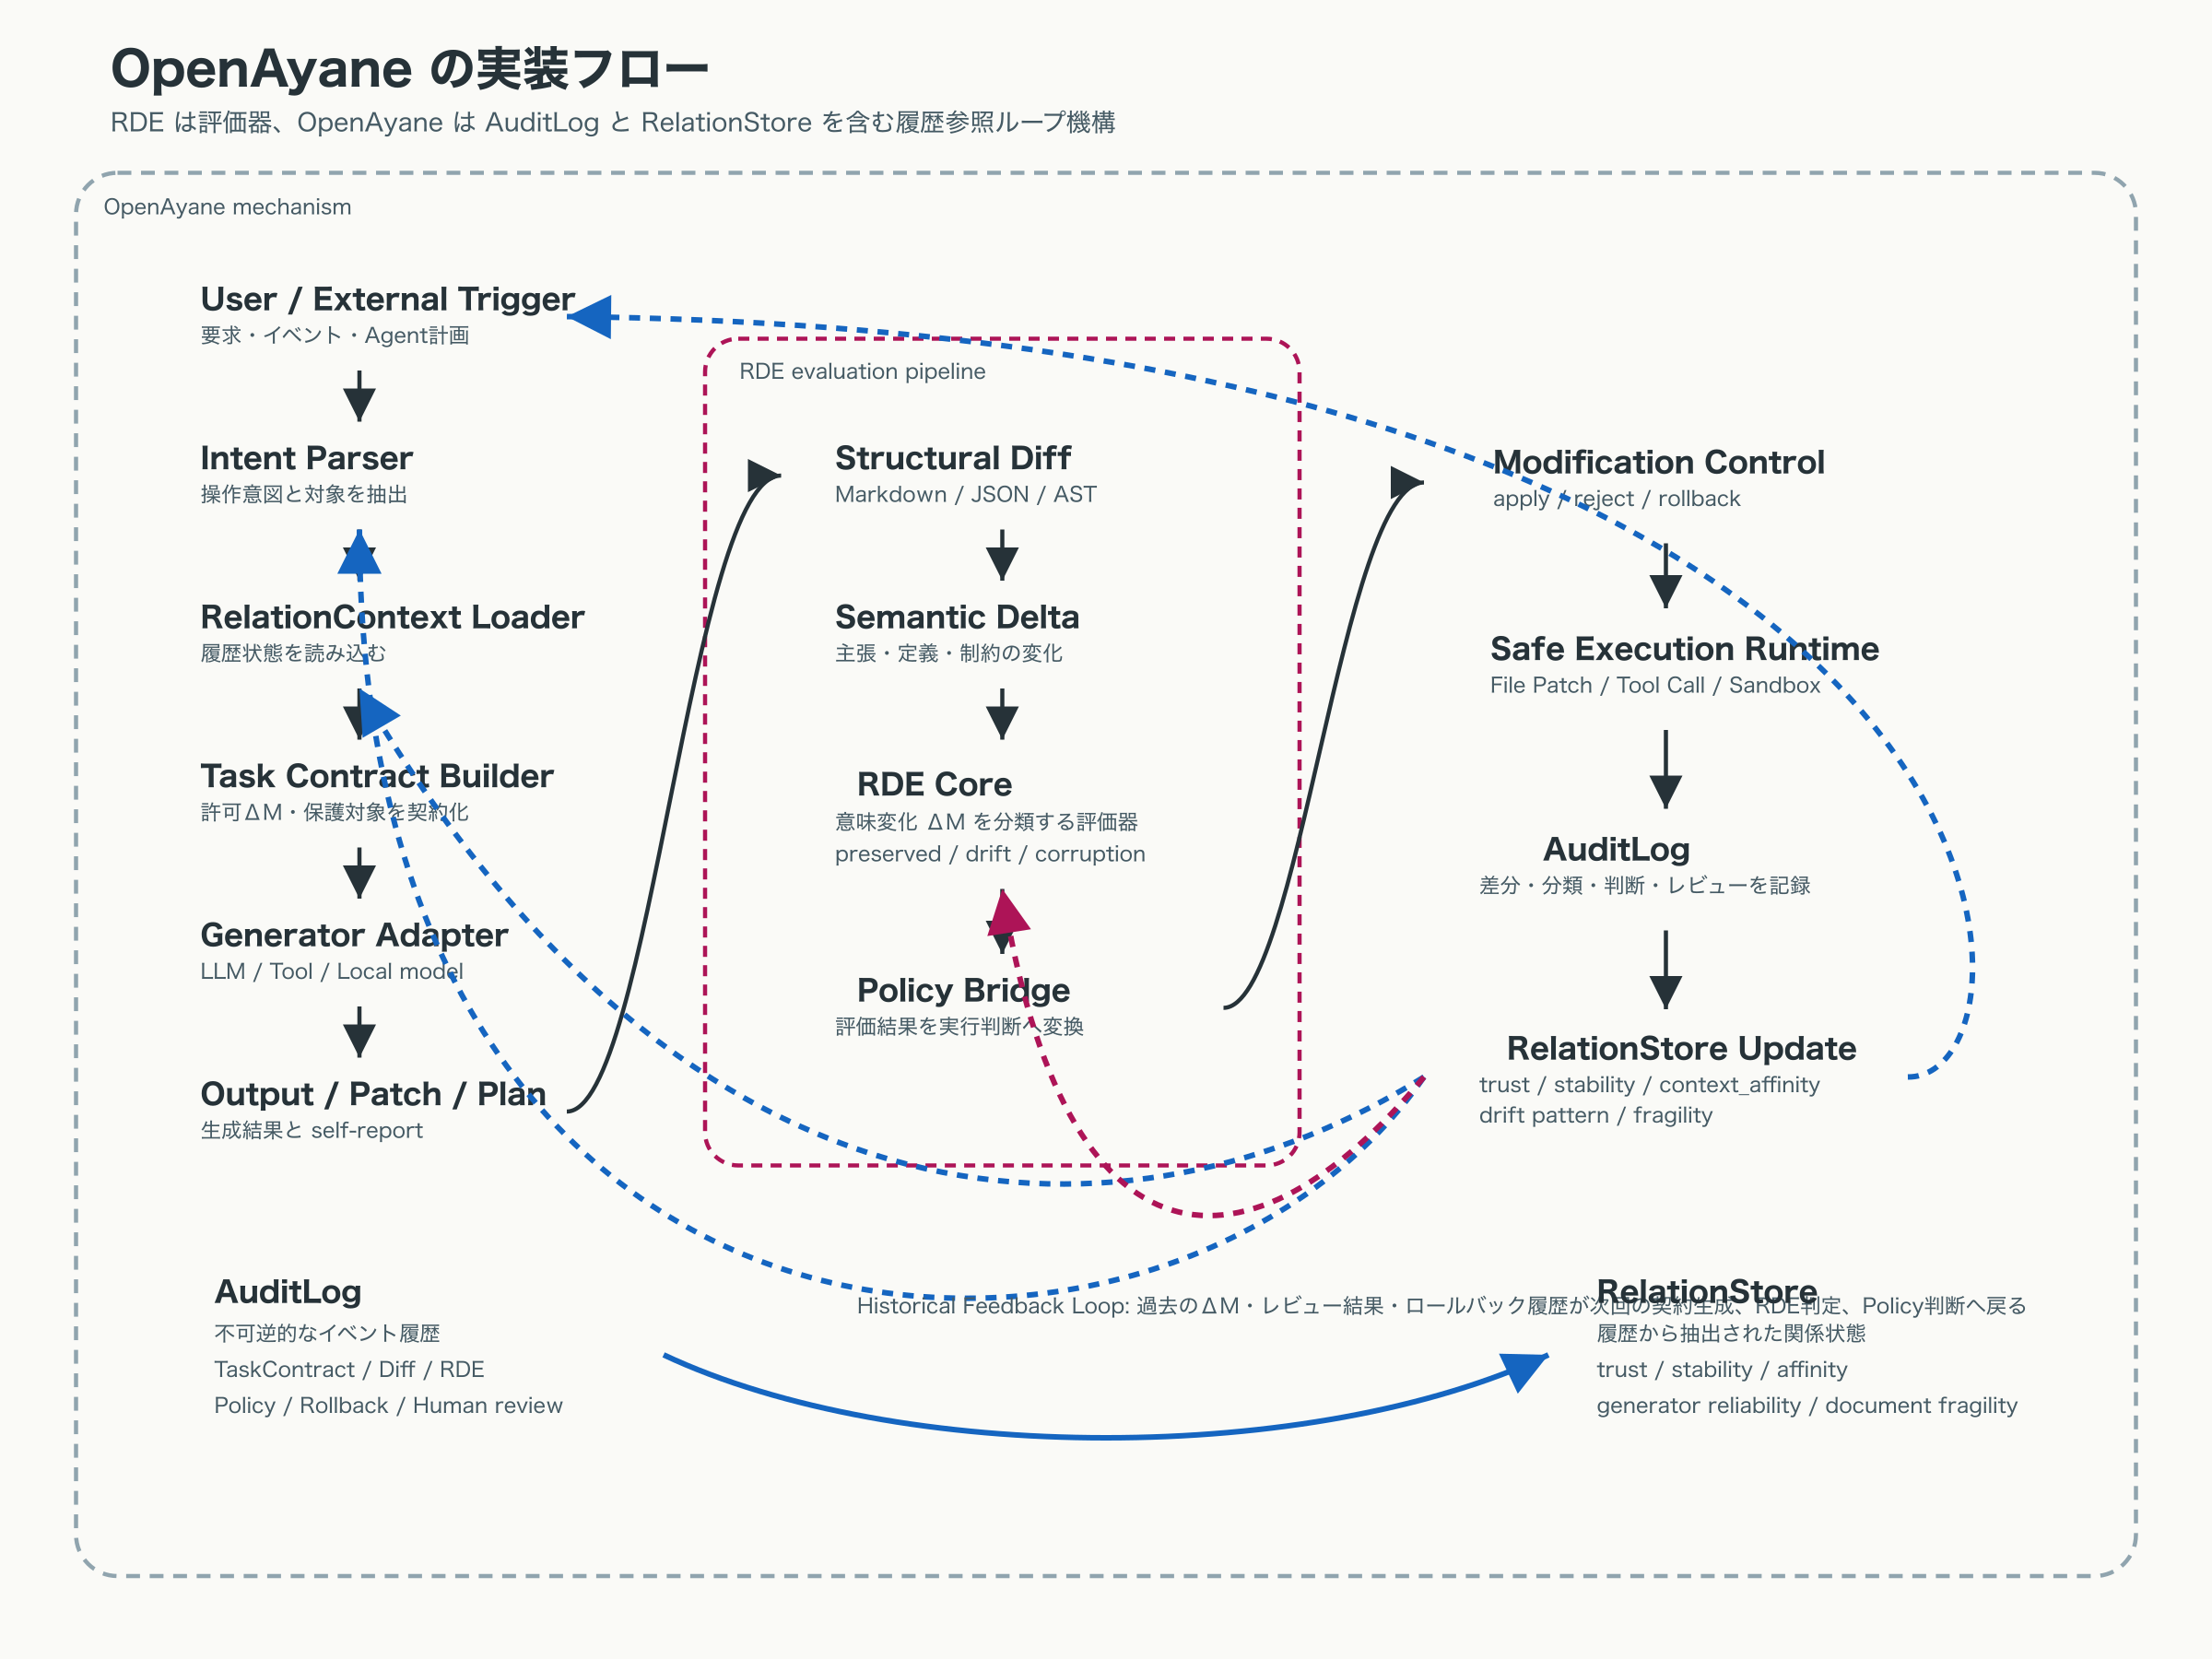
\includegraphics[width=0.96\linewidth]{openayane_implementation_flow.png}
  \caption{OpenAyaneの実装フロー。RDEは意味変化$\Delta M$を分類する評価器であり、OpenAyaneはTask Contract生成、生成器制御、差分抽出、RDE評価、Policy判断、実行制御、AuditLog、RelationStore更新、履歴参照ループを統合する機構である。}
  \label{fig:openayane-implementation-flow}
\end{figure}

\section{主要モジュール}
OpenAyaneは、Intent Parser、RelationContext Loader、Task Contract Builder、Generator Adapter、Structural Diff Engine、Semantic Delta Engine、RDE Core、Policy Bridge、Modification Control Flow、Safe Execution Runtime、AuditLog、RelationStoreから構成される。

\subsection{Task Contract}
Task Contractは、曖昧な自然言語指示を、RDEが評価可能な契約へ変換する。許可された$\Delta M$、禁止された$\Delta M$、保護対象、出力形式、レビュー方針を明示することで、Generatorの出力とRDEの評価基準を同時に規定する。

\subsection{RDE Core}
RDE Coreは、Semantic DeltaをTask Contract、Policy、Relation Stateと照合し、逸脱分類と推奨アクションを出す。ただし、RDEのrequired actionは最終決定ではなく、Policy Bridgeへの推奨である。最終的な承認、差し戻し、停止、ロールバックはPolicy Bridgeが行う。

\subsection{AuditLogとRelationStore}
AuditLogは、過去に何が起きたかの不可逆的記録である。RelationStoreは、その履歴から抽出された関係状態である。両者を分離することで、OpenAyaneは単発の安全フィルタではなく、意味変化の履歴を通じて判断条件を更新する関係的制御ループとなる。

\section{段階的実装計画}
Phase 0では、RDE定義、Task Contract、逸脱分類、OpenAyane既存モジュールとの対応を固定する。Phase 1では、Markdown、JSON、Pythonを対象とするStructural RDE MVPを実装する。Phase 2ではSemantic Delta EngineとRelationStore更新を導入する。Phase 3ではAgent Execution Gateを統合し、ツール実行前後の意味変化と権限を評価する。Phase 4ではInstitution Layerへ接続し、PoP-UID、組織Policy、外部監査、規範レジストリと連携する。

\section{評価計画}
評価は、生成品質ではなく、意味変化の検出、分類、承認制御、監査可能性、長期安定性を対象とする。Unit Test、Golden Test、Adversarial Test、Long-chain Test、Human Review Calibrationを用いる。特に、Unauthorized Change Detection Rate、Critical Corruption Recall、Generator Self-report Mismatch Detection Rate、Long-chain Semantic Drift Detection Rateを重視する。

\section{RDE差異検証}
本稿は、OpenAyane / RDE設計思想および基本設計からの変換結果である。保存された要素は、RDEがDiff、Policy、LLM Evaluatorそのものではなく、意味逸脱を裁定する評価器であるという定義である。変換された要素は、実装設計を研究論文として読める構造へ再配置した点である。補完された要素は、RDEとOpenAyaneの役割分担、履歴参照ループ、評価計画、非機能要件である。未解決の要素は、context\_affinityの厳密な更新式、Semantic Deltaの信頼性、Human Review Calibrationの具体的データセット、Institution Layerの制度設計である。

\section{結論}
OpenAyaneは、RDEを中核評価器として含む意味変化監査機構である。RDEは意味変化を分類する。OpenAyaneは、その評価結果を実行制御、監査、履歴更新、次回判断へ接続する。したがってOpenAyaneの核心は、単発の出力審査ではなく、AuditLogとRelationStoreを通じて過去の$\Delta M$を読み、現在の変換を評価し、未来の許可条件を更新する関係的制御ループにある。

\begin{thebibliography}{9}
\bibitem{Kano2026Resonanceverse}
Kano, Tomoyuki. 2026. \textit{意味の非収束と共鳴条件：誤配に基づく Resonanceverse の基礎理論}. Version 1.2. Zenodo. DOI: \href{https://doi.org/10.5281/zenodo.20016805}{10.5281/zenodo.20016805}.

\bibitem{Lewis2020RAG}
Lewis, Patrick, et al. 2020. ``Retrieval-Augmented Generation for Knowledge-Intensive NLP Tasks.'' arXiv:2005.11401.

\bibitem{Ouyang2022RLHF}
Ouyang, Long, et al. 2022. ``Training Language Models to Follow Instructions with Human Feedback.'' \textit{Advances in Neural Information Processing Systems}.

\bibitem{Yao2022ReAct}
Yao, Shunyu, et al. 2022. ``ReAct: Synergizing Reasoning and Acting in Language Models.'' arXiv:2210.03629.

\bibitem{Wilkinson2016FAIR}
Wilkinson, Mark D., et al. 2016. ``The FAIR Guiding Principles for Scientific Data Management and Stewardship.'' \textit{Scientific Data} 3:160018.
\end{thebibliography}

\end{document}
